
% This LaTeX was auto-generated from MATLAB code.
% To make changes, update the MATLAB code and republish this document.

\documentclass{article}
\usepackage{graphicx}
\usepackage{color}

\sloppy
\definecolor{lightgray}{gray}{0.5}
\setlength{\parindent}{0pt}

\begin{document}

    
    \begin{verbatim}
n=[10,30,50];
theta=2.2;

Counter=1;
mle=zeros(3,1);

figure
while Counter<=3
    u=rand(n(Counter),2);
    x=-log(1-u(:,1))/theta-log(1-u(:,2))/theta;
    %Produces a latex table
    %latex(sym(vpa(x)))
    mle(Counter)=2*n(Counter)/sum(x);

    %Plots the log likelihood function
    t=linspace(0,5);
    y=loglike(x,t,n(Counter));
    plot(t,y)
    hold on
    Counter=Counter+1;
end

xlabel("\theta")
ylabel("Log Likelihood Function")
legend('n=10','n=30','n=50')
print('Image_7_1','-depsc')

disp(mle)

function answer=loglike(x,t,n)
    count=1;
    answer=1;
    while count<=n
        answer=answer.*g(x(count),t);
        count=count+1;
    end
    answer=log(answer);
end

function answer=g(x,t)
    answer=t.^(2)*x.*exp(-t*x);
end
\end{verbatim}

        \color{lightgray} \begin{verbatim}           1.7781356231776
          2.68126943439986
          2.88130514300037

\end{verbatim} \color{black}
    
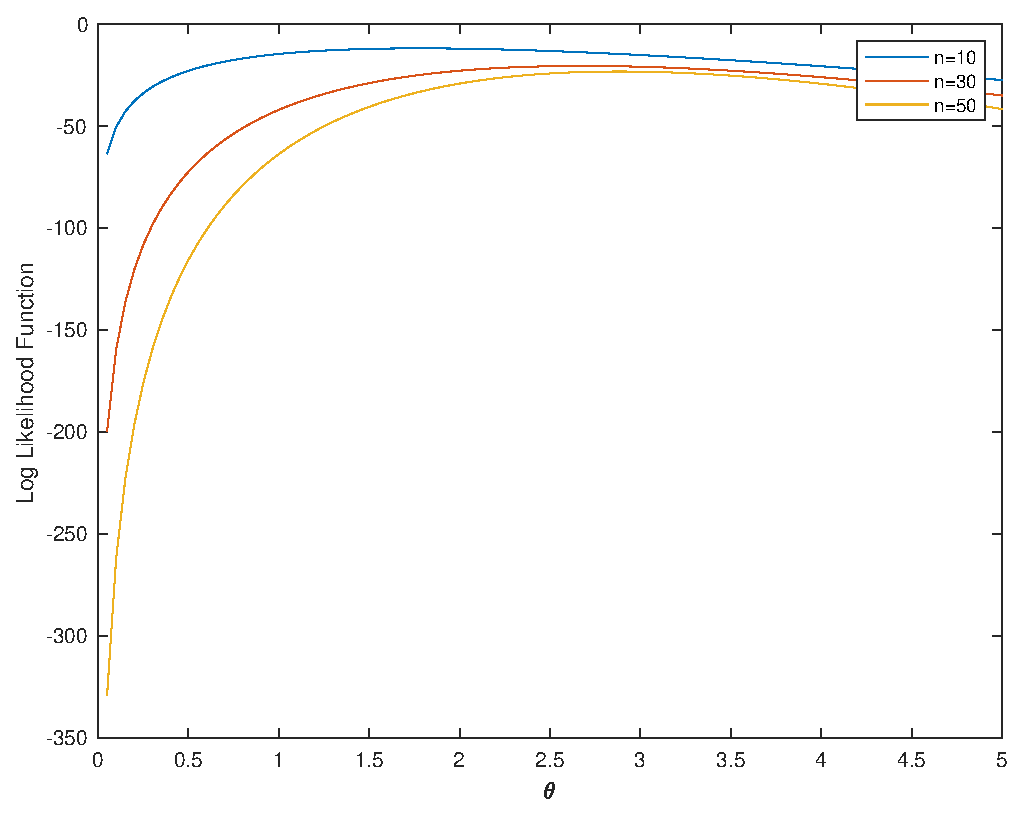
\includegraphics [width=4in]{Code_7_1_01.eps}



\end{document}
    
